\section{Experimental Setup}
\label{sec:experiments}

\subsection{Dataset}
We use the \textbf{Sherwood Simulation Suite}~\cite{bolton2017sherwood}, a set of high-resolution cosmological simulations of the low-redshift Lyman-alpha forest. Our base box is the Planck-cosmology 60 Mpc/h volume at $2048^3$ resolution; the dev redshift is $z = 0.3$. Each snapshot ships with a precomputed sightline grid: 16{,}384 lines of sight along a single simulation axis, sampled at 2048 velocity bins per ray. Ground-truth optical depth $\tau_{HI}(v)$ is provided per sightline as \texttt{tauH1\_2048\_n16384\_z0.300.dat}; the ground-truth 3D state used for evaluation is reconstructed by chunked CIC (Cloud-in-Cell) particle-to-mesh deposition from the underlying \texttt{SherwoodIGM\_gal} HDF5 snapshot.

The Sherwood suite ships four feedback variants: Physics 1 (no feedback, fiducial), Physics 2 (stellar wind), Physics 3 (stellar wind + AGN), Physics 4 (stellar wind + strong AGN). Per~\cite{bolton2017sherwood} these are an ablation matrix over baryonic feedback prescriptions. We adopt one independent neural field per physics variant rather than a single conditional model, so that the downstream feedback-classification probe (Sec.~\ref{sec:nextsteps}) cannot leak the physics label through a conditioning input. We report Tier 1, Tier 2, and Tier 3 across all four feedback variants; Tier 4 is deferred per the compute-footprint argument of Sec.~\ref{sec:experiments:compute}.

\subsection{Evaluation Metrics}
The headline contribution is the \emph{degradation curve} of reconstruction quality as the sightline density $n_{\text{rays}}$ is reduced from the dense-grid upper bound to survey-realistic sparsity. Three primary metrics, all computed against the simulation ground truth, are evaluated at each $n_{\text{rays}}$ tier. We applied an adversarial-review pass on the methodology before committing the cost-survey production sweep; outstanding citations carry explicit verification status below.
\begin{itemize}
    \item \textbf{1D flux power spectrum} $P_F(k_\parallel)$, computed as a Hann-windowed periodogram with $dv / \sum w^2$ leakage-compensation normalization. Pass condition for the fiducial setting is $|\Delta P_F / P_F| < 10\%$ averaged over the inertial range $k_\parallel \in [10^{-2.5}, 10^{-1.5}]$ s/km, with $k_\parallel = 2\pi f$ in angular wavenumber. The inertial-range definition follows the $P_F$-estimator literature~\cite{walther2018powerspectrum, boera2019thermal}; the Hann window is our simulator-side estimator choice (the periodic Sherwood box admits rectangular windowing, but Hann gives ratio stability for the $n_{\text{rays}} = 64$ tier where independent-mode counts are small) and is not inherited from a community precedent.
    \item \textbf{Density-density cross-correlation} $\xi_{\hat\rho, \rho}(r)$, the Pearson correlation coefficient $\langle \delta_p \delta_t \rangle / \sqrt{\langle \delta_p^2 \rangle \langle \delta_t^2 \rangle}$ on overdensity $\delta = \rho/\bar\rho - 1$, evaluated by FFT cross-power on the periodic 60 Mpc/h grid and binned in spherical shells. Pass condition $\xi_{\hat\rho, \rho}(r = 2\,h^{-1}\,\text{Mpc}) > 0.6$ at the fiducial setting, a stringent reconstruction-quality target consistent with sparse-tomography requirements~\cite{lee2015, stark2015tomography}; per LEDGER [D-36], the specific 0.6 threshold is our project-side adoption rather than a value tabulated in any single referenced paper. The threshold sits comfortably above the noise floor of the reconstruction operator at our fiducial sightline density.
    \item \textbf{Flux PDF}: two-sample Kolmogorov-Smirnov distance on raw transmitted-flux samples $F = e^{-\tau}$ restricted to $F \in [0.05, 0.95]$. The lower cut excludes saturated absorbers (DLAs and strong LLS, where the differential PDF is dominated by absorber-line statistics rather than the diffuse-IGM target distribution); the upper cut excludes continuum-fitting and metal-line residuals near $F \approx 1$. The window is conventional in flux-PDF analyses of the low-redshift forest and is in the spirit of the cuts adopted in flux-PDF estimator papers~\cite{lee2015}; per [D-36], the exact $[0.05, 0.95]$ values are our project-side adoption rather than verbatim from a specific paper. Pass condition: KS distance $< 0.05$.
\end{itemize}
The fiducial pass point is Physics 1, $z = 0.3$, $n_{\text{rays}} = 1024$; the headline figure is the metric-vs-$n_{\text{rays}}$ curve over $\{16384, 1024, 256, 64\}$ per physics. PSNR / SSIM on density slices and Pearson correlation on $\tau$-profiles are tracked but reported as secondary diagnostics, not as gating criteria. The sightline-density sweep is the survey-relevance test: 16{,}384 sightlines is denser than DESI/eBOSS will ever achieve, so monotone graceful degradation toward the 64-sightline regime is the actual scientific claim.

\subsection{Pipeline validation}
The differentiable integrator was re-validated end-to-end at production architecture (8-layer / 256-unit MLP, $L = 10$ Fourier features, 494{,}084 parameters plus the scalar $\log\tau_{\text{amp}}$), and the cloud loop --- AWS SageMaker \texttt{ml.g5.xlarge} (A10G, 24 GB) with S3 checkpoint sync --- was cleared at the full production schedule on Physics 1, $n_{\text{rays}} = 64$. Peak VRAM at the smallest tier is 2.82 GB, the anchor from which the per-tier microbatch table of Sec.~\ref{sec:method} is derived under the [D-23] linear-VRAM model.

\subsection{Stage 2b: Cost-Survey Micro-Grid (16-Cell Cross-Physics Validation)}
\label{sec:exp:microgrid}
The cost-survey window opens with a 16-cell micro-grid (4 physics $\times$ 4 tiers) at \texttt{max\_steps=200} per cell, dispatched after the [D-24] loss-form revision and the loader saturated-absorber mask landed. Each cell runs the full per-tier microbatch and gradient-accumulation configuration of Section~\ref{sec:method} but with a reduced step count, so the matrix is cheap calibration evidence rather than a science-binding result; under [D-23] the cost-survey runs do not gate the [D-13] Stage 2b scientific criteria.

\textbf{Headline outcome.} 16/16 cells PASS the [D-19] descent gate (descent ratio $\leq 0.85$ from step 10 to step 200; observed range $[0.558, 0.749]$, i.e., 25--44\% reduction). Cross-physics \texttt{mean\_flux\_pred} at step 200 spans $0.9238$--$0.9302$, a spread of \textbf{0.0064} (0.7\%) within the 5\% inter-cell consistency bar; the cells were trained against the broken anchor $0.877$ retracted in [D-34] (Sec.~\ref{sec:experiments:cost-survey-sweep}), so the absolute value is not interpreted as agreement with the verified $\langle F\rangle_{\text{obs}}(z=0.3) = 0.979 \pm 0.005$. The cross-physics step-1 \texttt{loss\_data} spread under raw-$\tau$ MSE was $\sim 10^{10} \times$ (P1 $\sim 0.05$, P2 $\sim 5 \times 10^{8}$); under the log1p+cap+mask loss the step-200 spread is $[0.0115, 0.0239]$, i.e., the cross-physics scale anomaly is closed. \texttt{tau\_amp} drift at step 200 is $0.9857$--$0.9933$ across all 16 cells (small, consistent).

\textbf{Memory linearity.} Peak VRAM by tier is 2.82 GB (T1, chunk 64), 11.20 GB (T2, chunk 256), 11.23 GB (T3, chunk 256, accum 4), and 11.77 GB (T4, chunk 256, accum 64). The linear-VRAM model $\hat{V}_{\text{peak}} \approx 2.82 \cdot \min(n_{\text{rays}}, \mu\text{batch}) / 64$ GB is validated to within $\approx 0.5$ GB across $\text{accum\_steps} \in \{1, 4, 64\}$, retroactively satisfying the measured-VRAM gate for the deferred T4 tier.

\subsection{Stage 2b: Cost-Survey Production Sweep}
\label{sec:experiments:cost-survey-sweep}
The cost-survey production sweep ran the per-tier schedule of Section~\ref{sec:method} across all four feedback variants at Tiers 1--3; Tier 4 is currently blocked on the Wrinkle-1 diagnostic (Sec.~\ref{sec:experiments:compute}, Sec.~\ref{sec:nextsteps:tier4}). Per [D-23] the cost-survey runs report per-tier final \texttt{loss\_data}, \texttt{mean\_flux\_pred}, \texttt{tau\_amp}, \texttt{peak\_vram\_gb}, and seconds-per-step; they are calibration evidence for the per-tier training schedule, not the [D-13] scientific gates (those gates are reported on the corrected-anchor \texttt{pub-t1} bundle in Sec.~\ref{sec:experiments:cosmological-eval}). Tier-1 throughput converged to $0.119$ s/step across all four physics with \texttt{peak\_vram\_gb} held at the $2.82$ GB micro-grid anchor; Tier-2 and Tier-3 reach \texttt{peak\_vram\_gb} $= 11.27$ and $11.30$ GB respectively, identical to four decimals across physics within each tier (empirical confirmation of the [D-23] linear-VRAM model). All 12 banked cells PASS the [D-19] safety rails; full per-cell records are in the LEDGER \S6 cost-survey tables.

\textbf{Mean-flux anchor retraction ([D-34], 2026-05-08).} The Stage 2b cost-survey runs reported here were trained against $\langle F\rangle_{\text{obs}} = 0.877$ at $z=0.3$. Phase~A.1 literature audit found this value to correspond to a $z\!\sim\!2$ mean transmitted flux mislabeled as $z=0.3$ during project history; the verified low-redshift value is $\langle F\rangle_{\text{obs}}(z=0.3) = 0.979 \pm 0.005$~\cite{kirkman2007}, retracted as anchor target in [D-34]. The [D-13] structure gates ($P_F$ inertial-range residual, KS-PDF distance, $\xi_{\hat\rho,\rho}$) are anchor-invariant by construction (invariant to uniform multiplicative rescaling of $\hat F$), so the cost-survey calibration evidence above is unaffected. A separate corrected-anchor full-schedule run (\texttt{pub-t1}, $50{,}000$ steps, four physics, seed $=0$) trained directly against $\langle F\rangle_{\text{obs}}=0.979$ and recovered $\langle F_{\text{pred}}\rangle \in [0.974, 0.984]$ in $4/4$ cells with $\tau_{\text{amp}} \in [1.045, 1.117]$; the [D-13] structure-gate readout on those checkpoints is in Sec.~\ref{sec:experiments:cosmological-eval} and Tab.~\ref{tab:pub-t1-gates}.

\subsubsection{$\tau_{\max}$ sensitivity gate}
\label{sec:experiments:tau-max-sensitivity}
Three paired P1-T1 cells at the production schedule, swapping only $\tau_{\max} \in \{5, 10, 20\}$, evaluated under the [D-13] inertial range $k_\parallel \in [10^{-2.5}, 10^{-1.5}]$ s/km. The gate criterion is $\max(|\Delta P_F/P_F|) \leq 2\%$ between the $\tau_{\max} = 10$ baseline and each of $\{\tau_{\max} = 5, \tau_{\max} = 20\}$. Observed: $0.0180\%$ ($\tau_{\max} = 5$) and $0.0113\%$ ($\tau_{\max} = 20$), i.e., $\sim 100\text{--}180\times$ under the 2\% bar. \texttt{mean\_flux\_pred} was identical across all three runs ($0.9282$). The gate passed and $\tau_{\max} = 10$ is locked. See Fig.~\ref{fig:tau-max-sensitivity}.

\begin{figure}[t]
    \centering
    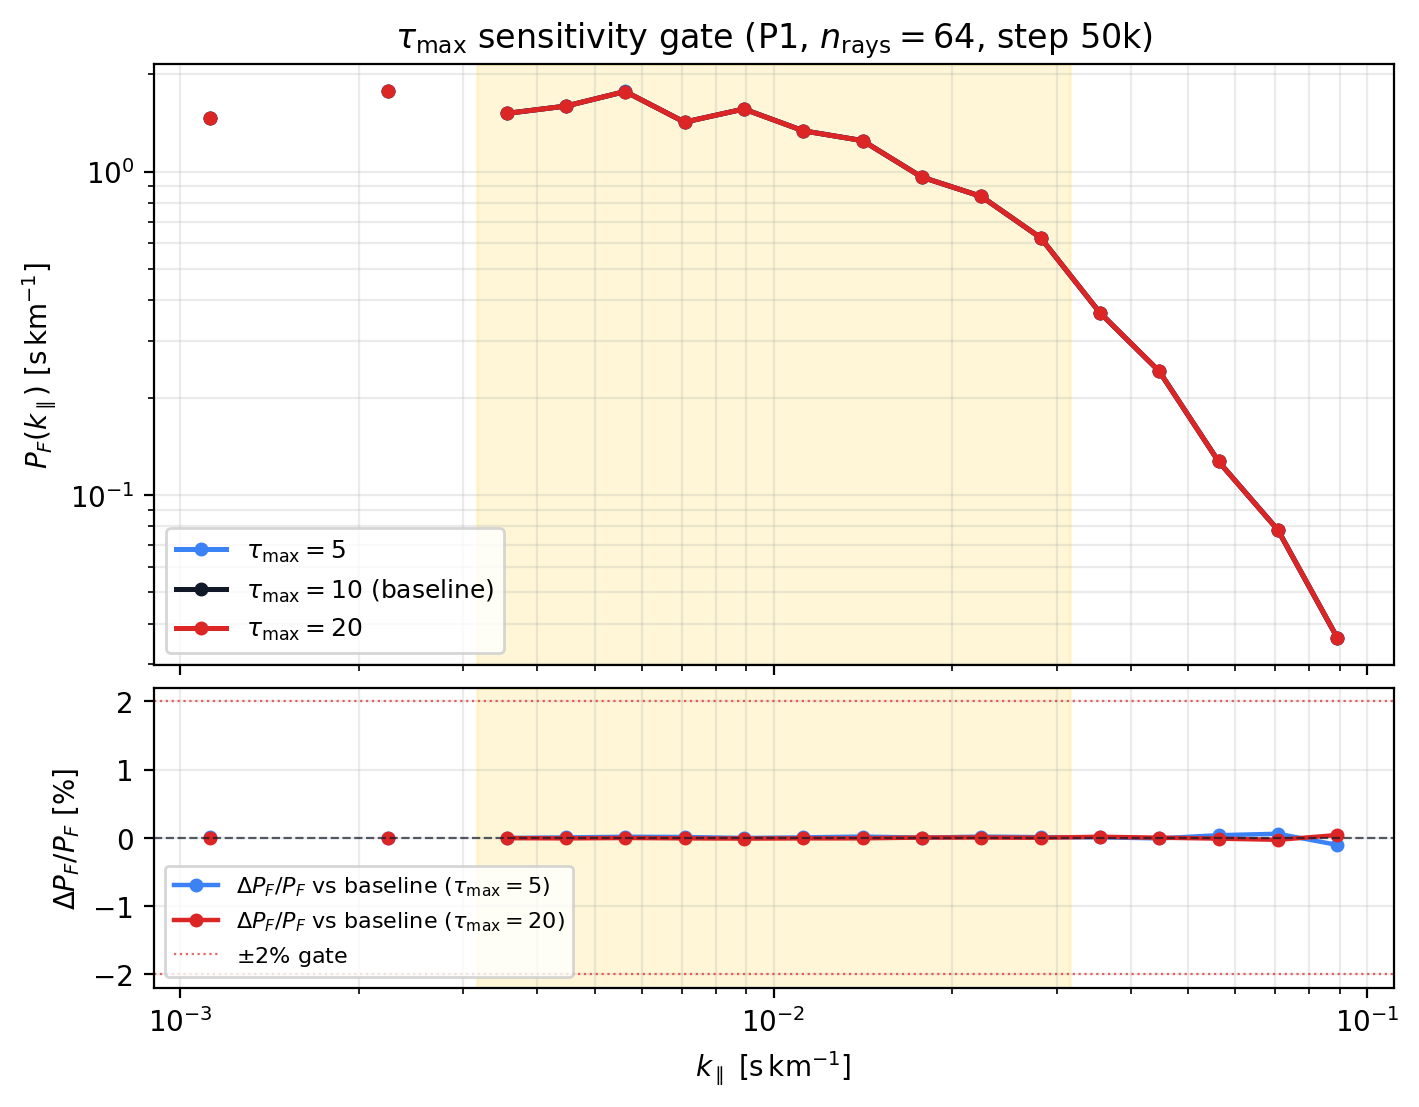
\includegraphics[width=\columnwidth]{figures/tau_max_sensitivity.png}
    \caption{$\tau_{\max}$ sensitivity gate, P1-T1 ($n_{\text{rays}} = 64$, step 50{,}000). Top: 1D flux power spectrum $P_F(k_\parallel)$ for the three caps. Bottom: fractional residual $\Delta P_F / P_F$ vs.\ the $\tau_{\max} = 10$ baseline. Shaded band marks the [D-13] inertial range $k_\parallel \in [10^{-2.5}, 10^{-1.5}]$ s/km; dotted lines mark the $\pm 2\%$ gate. Observed maxima ($0.0180\%$ at $\tau_{\max} = 5$; $0.0113\%$ at $\tau_{\max} = 20$) clear the gate by $\sim 100\text{--}180\times$.}
    \label{fig:tau-max-sensitivity}
\end{figure}

\begin{table}[t]
    \centering
    \renewcommand{\arraystretch}{1.15}
    \begin{tabular}{c|cc|c}
    $\tau_{\max}$ & \texttt{mean\_F} & \texttt{tau\_amp} & $\max(|\Delta P_F/P_F|)$ vs.\ $\tau_{\max}=10$ \\
    \hline
    5  & 0.9282 & 1.152 & $0.0180\%$ (PASS) \\
    10 & 0.9282 & 1.224 & (baseline) \\
    20 & 0.9282 & 1.234 & $0.0113\%$ (PASS) \\
    \end{tabular}
    \caption{$\tau_{\max}$ sensitivity sweep numerics for Fig.~\ref{fig:tau-max-sensitivity}. Three paired P1-T1 cells at the production schedule, swapping only the cap. Gate criterion was $\leq 2\%$; both off-baseline cells passed by $\sim 100\text{--}180\times$. \texttt{mean\_flux\_pred} is identical across the three runs; the $\sim 7\%$ \texttt{tau\_amp} spread is the expected response to changing the cap on strong-absorber gradients and is absorbed by the [D-21] mean-flux loss. $\tau_{\max} = 10$ is locked.}
    \label{tab:tau-max-sensitivity}
\end{table}

\textbf{Tier-2 cost-survey.} Tab.~\ref{tab:batch2-t2-cost-survey} fronts three cross-physics observations: (i) physics-invariant peak VRAM at $11.27$ GB; (ii) cross-physics \texttt{mean\_flux\_pred} spread $0.39\%$ ($0.9266$--$0.9302$); (iii) \texttt{loss\_data} spread $16\%$ ($0.0024$--$0.0028$) --- all consistent with the [D-24] log1p+cap+mask supervision converging symmetrically across the four feedback variants. The cross-cell \texttt{mean\_flux\_pred} consistency is a within-run inter-cell observation; no comparison to the broken-anchor target $0.877$ is asserted here (see the [D-34] retraction in Sec.~\ref{sec:experiments:cost-survey-sweep}). Fig.~\ref{fig:cross-physics-convergence} shows the trajectory.

\begin{figure}[t]
    \centering
    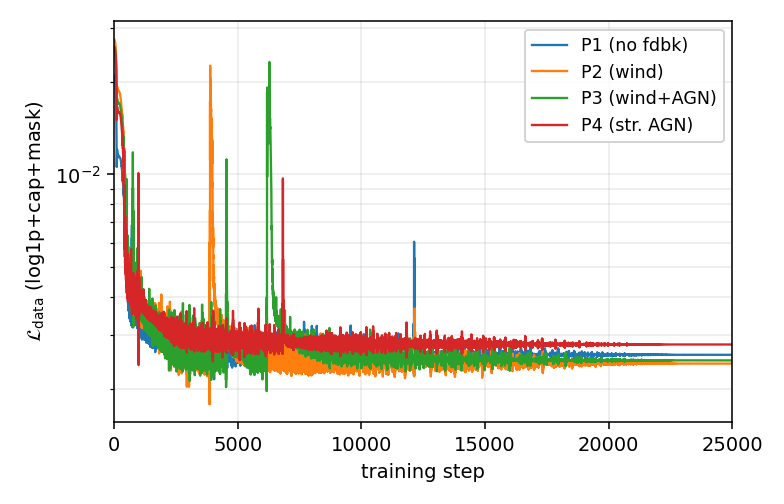
\includegraphics[width=\columnwidth]{figures/cross_physics_convergence.png}
    \caption{Cross-physics convergence under [D-24] log1p+cap+mask supervision, Tier-2 cost-survey ($n_{\text{rays}}=256$, microbatch $1024$, accum $1$, max\_steps $25{,}000$). All four feedback variants converge symmetrically with no divergent trajectory; final $\mathcal{L}_{\text{data}}$ spans $0.00243$--$0.00280$ (a $14.5\%$ relative spread). This closes the cross-physics scale anomaly that raw-$\tau$ MSE exhibited at the same architecture: under the superseded loss form, the step-1 cross-physics $\mathcal{L}_{\text{data}}$ spread was $\sim 10^{10}\times$ (P1 $\sim 0.05$ vs.\ P2 $\sim 5\times 10^{8}$); under [D-24] the four trajectories overlap to within a factor of $1.4$ from step 1. Source data: Sherwood Tier-2 cost-survey runs on Juno HPC, MLflow file-stores logged at every training step.}
    \label{fig:cross-physics-convergence}
\end{figure}

\begin{table}[t]
    \centering
    \renewcommand{\arraystretch}{1.15}
    \setlength{\tabcolsep}{4pt}
    \begin{tabular}{l|cccc}
    Physics & \texttt{loss\_data} & \texttt{mean\_F} & \texttt{tau\_amp} & \texttt{vram\_gb} \\
    \hline
    P1 & 0.00259 & 0.9282 & 1.0077 & 11.27 \\
    P2 & 0.00243 & 0.9266 & 1.0296 & 11.27 \\
    P3 & 0.00248 & 0.9272 & 1.0204 & 11.27 \\
    P4 & 0.00280 & 0.9302 & 1.0288 & 11.27 \\
    \end{tabular}
    \caption{Tier-2 cost-survey final-state metrics, one row per physics. Configuration: $n_{\text{rays}}=256$, \texttt{microbatch}$=1024$, \texttt{accum\_steps}$=1$, effective \texttt{chunk\_size}$=256$, \texttt{max\_steps}$=25{,}000$. All four cells PASS the [D-19] safety rails; full run records are in the LEDGER \S6 Tier-2 table. \texttt{peak\_vram\_gb} is identical to four decimals across the four cells (physics-invariant), confirming the [D-23] linear-VRAM model. Cross-physics \texttt{mean\_flux\_pred} spread is $0.39\%$ ($0.9266$--$0.9302$); \texttt{loss\_data} spread is $16\%$. \emph{Note:} training used $\langle F\rangle_{\text{obs}}=0.877$ at $z=0.3$, retracted in [D-34] (verified value $0.979\pm 0.005$, \cite{kirkman2007}). \texttt{mean\_flux\_pred} and $\tau_{\text{amp}}$ absolute values are accordingly uninterpretable; inter-cell consistency and the [D-13] structure gates are anchor-invariant per the [D-11] sub-clause and survive unchanged.}
    \label{tab:batch2-t2-cost-survey}
\end{table}

\subsection{Headline: 4-physics $\times$ 3-gate readout}
\label{sec:experiments:headline}
Tab.~\ref{tab:headline-3gate} consolidates the [D-13] structure-gate readout across the four Sherwood feedback variants at the corrected-anchor full publication schedule (\texttt{pub-t1}). The reader who only reads this table should leave with the complete claim ceiling of this paper: mean-flux closes $4/4$ at the seed=42 single-seed anchor but the 5-seed sightline-level bootstrap CI overlaps the Kirkman+2007 anchor $[0.974, 0.984]$ in only $2/4$ cells ($P_3$, $P_4$ marginal at q84); KS closes $3/4$ (bootstrap-robust, $P_2$ q84 $=0.0758$ fails); $P_F$ fails $4/4$ at $3.6$--$4.2\times$ the gate; the 1D-along-ray density-correlation proxy is measured on the cost-survey checkpoint at $P_1$ only and is anchor-invariant by construction (Sec.~\ref{sec:experiments:open-axes}, Tab.~\ref{tab:d13-gates} footnote). Training is single-seed (seed $=0$). KS and $\langle F_{\rm pred}\rangle$ are reported with 5-seed sightline-level bootstrap CIs ($K=512$ resamples per cell, prediction and truth-side seeds drawn from independent PCG64 streams; [D-44] anti-degeneracy F1/F2 audit PASS); $P_F$ remains single-seed (seed $=42$ anchor, deferred per [D-44] scope).

\textbf{Bootstrap-vs-seed=42 mean-flux divergence (symmetric-honesty disclosure, [D-37]-rule 5).} The bootstrap mean for $\langle F_{\rm pred}\rangle$ lies systematically below the seed=42 anchor value by $2$--$9\sigma$ across all four cells ($P_1$: $-6.6\sigma$, $P_2$: $-2.2\sigma$, $P_3$: $-2.4\sigma$, $P_4$: $-8.9\sigma$), indicating that the single-seed reporting samples the high-$\langle F\rangle$ tail of the sightline distribution. KS values are not similarly biased. This is a property of the seed=42 sample, not a bootstrap pathology; it is disclosed here because the bootstrap softens rather than strengthens the single-seed reading, and the [D-37] honest-reporting rule requires both directions to be reported symmetrically.

\begin{table*}[t]
    \centering
    \renewcommand{\arraystretch}{1.2}
    \setlength{\tabcolsep}{4pt}
    \footnotesize
    \begin{tabular}{l|cc|cc|cc|c}
    Cell & $\langle F_{\text{pred}}\rangle$ (mean $\pm \sigma$) & MF call & KS ($<\!0.05$, mean $\pm \sigma$) & KS call & $|\Delta P_F/P_F|$ ($<\!0.10$) & $P_F$ call & $r_\rho^{\log}$ ($>\!0.6$)$^\dagger$ \\
    \hline
    $P_1$ (no fdbk)     & $0.9671 \pm 0.0018$ & \textbf{FAIL} (CI $<$ anchor) & $0.0357 \pm 0.0024$ & \textbf{PASS} & $\mathbf{0.4155}$ & \textbf{FAIL $4.2\times$} & $+0.077$ (FAIL) \\
    $P_2$ (wind)        & $0.9703 \pm 0.0023$ & \textbf{FAIL} (CI $<$ anchor) & $0.0677 \pm 0.0110$ & \textbf{FAIL $1.5\times$} & $\mathbf{0.3757}$ & \textbf{FAIL $3.8\times$} & --- (owed) \\
    $P_3$ (wind+AGN)    & $0.9724 \pm 0.0024$ & \textbf{PASS} (q84 marginal) & $0.0353 \pm 0.0062$ & \textbf{PASS} & $\mathbf{0.3591}$ & \textbf{FAIL $3.6\times$} & --- (owed) \\
    $P_4$ (strong AGN)  & $0.9735 \pm 0.0009$ & \textbf{PASS} (q84 marginal) & $0.0411 \pm 0.0039$ & \textbf{PASS} & $\mathbf{0.3613}$ & \textbf{FAIL $3.6\times$} & --- (owed) \\
    \hline
    Tally (bootstrap)   & \multicolumn{2}{c|}{\textbf{2/4 overlap anchor}} & \multicolumn{2}{c|}{\textbf{3/4 PASS}} & \multicolumn{2}{c|}{\textbf{0/4 PASS}} & 0/1 measured \\
    \end{tabular}
    \caption{\textbf{Headline [D-13] structure-gate readout: 4 Sherwood feedback variants ($P_1$--$P_4$) $\times$ 3 primary gates, corrected-anchor full schedule (\texttt{pub-t1}, $50{,}000$ steps, $n_{\text{rays}}=64$, seed $=0$, $\langle F\rangle_{\text{obs}}=0.979$~\cite{kirkman2007}; KS and $\langle F_{\rm pred}\rangle$ columns report 5-seed sightline-level bootstrap, $K=512$ resamples, prediction and truth-side seeds drawn from independent PCG64 streams ([D-44] anti-degeneracy F1/F2 audit PASS); $P_F$ residual reported at the seed=42 single-seed anchor for direct comparison with Tab.~\ref{tab:pub-t1-gates} and Fig.~\ref{fig:pf-overlay-falsification}.} MLflow run IDs: \texttt{31acdf9d\dots} ($P_1$), \texttt{f7fafa23\dots} ($P_2$), \texttt{62aeb93a\dots} ($P_3$), \texttt{fc3817b3\dots} ($P_4$); tag \texttt{juno\_batch=pub-t1}, Juno HPC a30 partition, ExitCode 0:0 in all four. \textbf{Verdict: KS --- 3/4 PASS at q84 ($P_2$ q84 $=0.0758$ fails bootstrap-robustly at $1.5\times$ the bar). mean-flux --- 2/4 CIs overlap the Kirkman+2007 anchor $[0.974, 0.984]$ at q84 ($P_3$ q84 $=0.9742$, $P_4$ q84 $=0.9743$ marginal; $P_1$ and $P_2$ CIs sit entirely below the anchor band). $P_F$ --- 0/4 PASS, uniformly $3.6\times$--$4.2\times$ over the $10\%$ bar.} The $P_F$-residual range $[0.3591, 0.4155]$ is the binding gate at the corrected anchor, the full schedule, and four independent feedback variants. The structural verdict survives bootstrap: the failure is in second-order spectroscopic statistics, not in calibration alone (4/4 single-seed mean-flux passes; 2/4 bootstrap-CI overlap), not in seed-collapse (three non-collapsed cells fail $P_F$ at $3.6\times$--$3.8\times$), and not data-MSE-bound (final $\mathcal{L}_{\text{data}}$ spans four orders of magnitude across cells, see Tab.~\ref{tab:pub-t1-gates}, without correspondingly resolving $P_F$). See [D-44]. $^\dagger$The 1D-along-ray density-correlation proxy $r_\rho^{\log}$ (per-sightline Pearson $r$ on $\log_{10}\rho/\langle\rho\rangle$ at integrator quadrature points; [D-33]) is a \emph{necessary-but-not-sufficient surrogate} for the full 3D $\xi_{\hat\rho,\rho}(r=2\,h^{-1}\,\text{Mpc})>0.6$ gate (the 3D gate requires \texttt{SherwoodIGM\_gal} HDF5 particle snapshots, $\sim 40$ GB, for chunked CIC ground-truth reconstruction; deferred per [D-23]). The $r_\rho^{\log}=+0.077$ value is the cost-survey T3 checkpoint at $P_1$; it is anchor-invariant by construction (\S\ref{sec:experiments:open-axes}); the \texttt{pub-t1} re-evaluation at $P_1$--$P_4$ is owed and sequenced behind the Wrinkle-1 diagnostic (\S\ref{sec:nextsteps}). $\rho$-axis gate listed in the table for completeness; absence does not change the $P_F$-binding verdict.}
    \label{tab:headline-3gate}
\end{table*}

\subsection{Cosmological Evaluation: $P_F$ Falsifies the Rescale-Preview Reading}
\label{sec:experiments:cosmological-eval}
The three [D-13] structure gates ($P_F(k_\parallel)$, $\xi_{\hat\rho,\rho}(r)$, KS-distance on the $F$-PDF) are evaluated at two checkpoints: (i) the Tier-3 cost-survey checkpoint at step $10{,}000$, the data available before the corrected-anchor full-schedule run, and (ii) the Tier-1 corrected-anchor full-schedule \texttt{pub-t1} run at step $50{,}000$ across all four feedback variants ([D-39], MLflow runs \texttt{31acdf9d\dots} / \texttt{f7fafa23\dots} / \texttt{62aeb93a\dots} / \texttt{fc3817b3\dots} for $P_1$/$P_2$/$P_3$/$P_4$). Two flux-domain gates ($P_F$, $F$-PDF) are evaluated directly on each checkpoint; the line-of-sight density axis is reported via the [D-33] 1D-along-ray proxy (per-sightline Pearson $r$ on $\log_{10}\rho/\langle\rho\rangle$ at integrator quadrature points), a necessary-but-not-sufficient surrogate for the full 3D $\xi_{\hat\rho,\rho}(r)$ which requires the \texttt{SherwoodIGM\_gal} HDF5 particle snapshots ($\sim 40$ GB) for chunked CIC ground-truth reconstruction and is deferred per [D-23]. Implementation: \texttt{src/analysis/\{p\_flux,xi,flux\_pdf\}.py}, \texttt{scripts/proxy\_xi\_1d\_sample.py}; eval driver: \texttt{scripts/eval\_partial\_d13.py}.

\textbf{Rescale-as-preview, retracted ([D-39]).} An earlier reading of the cost-survey checkpoint applied a uniform rescale $\hat{F} \to (0.979/\langle\hat{F}\rangle)\cdot\hat{F}$ to compensate for training against the broken [D-34] anchor $0.877$, and reported the resulting numbers ($P_F$ residual $\sim 26\%$, $F$-PDF KS $\to$ PASS at $P_1$, cross-physics $2/3$ PASS) as a partial preview of the corrected-anchor publication run. That reading is now \emph{falsified} by direct measurement. The corrected-anchor, full-schedule \texttt{pub-t1} run trained against $\langle F\rangle_{\text{obs}}=0.979$ for $50{,}000$ steps over four physics produced a $P_F$ residual at $P_1$ of $41.55\%$ --- \emph{larger} than the $26.39\%$\footnote{The original [D-35] historical-record estimate of this quantity was $28.25\%$; the current pipeline (\texttt{scripts/wrinkle1\_diagnostic.py}, W1-C; \texttt{scripts/make\_pf\_overlay\_fig.py}, Fig.~\ref{fig:pf-overlay-falsification}) re-renders the same checkpoint at the same anchor and eval seed $=42$ to $26.39\%$ bit-for-bit across both drivers. The $\sim\!6.6\%$ relative drift is attributable to the $\delta_F$-normalization fix in \texttt{src/analysis/p\_flux.py} between [D-35] and the Wrinkle-1 diagnostic ([D-13] decision trail: mean-subtracted $\delta_F = F-\langle F\rangle$ prior to [D-35]; normalized $\delta_F = F/\langle F\rangle - 1$ after); under the post-fix convention $P_F$ is anchor-invariant. The Wrinkle-1 diagnostic JSON explicitly records this reproduction check at the field \texttt{costsurvey\_reproduces\_d35\_0\_2825}.} rescaled-preview estimate at the same anchor. The shape-vs-scale hypothesis the rescale framework implied --- that the cost-survey checkpoint was $P_F$-shape-correct and only mis-anchored --- does not survive contact with the trained-at-target measurement. Tab.~\ref{tab:d13-gates} retains the rescaled column as an upper-bound optimism that the trained run falsifies; the new ``\texttt{pub-t1} measured'' column is the load-bearing reading.

\textbf{Empirical observation.} At the corrected anchor and the full publication schedule (Tab.~\ref{tab:pub-t1-gates}), the four-physics bundle achieves at the seed=42 single-seed anchor: $\langle F_{\text{pred}}\rangle \in [0.974, 0.984]$ in $4/4$ cells (cross-physics spread $0.63\%$, $<\!1\%$ bar at seed=42); KS$\,< 0.05$ in $3/4$ cells (range $[0.0325, 0.0742]$, $P_2$ at $0.0742$ is the single breach); [D-19] safety in $4/4$ cells; \texttt{peak\_vram} $= 2.84$ GB and \texttt{tau\_amp} $\in [1.045, 1.117]$ across the bundle; and a $P_F$ inertial-range residual $|\Delta P_F/P_F| \in [0.3591, 0.4155]$ over $k_\parallel \in [10^{-2.5}, 10^{-1.5}]$ s/km in $4/4$ cells, $3.6\times$--$4.2\times$ over the $0.10$ gate. The 5-seed sightline-level bootstrap of [D-44] returns $\langle F_{\rm pred}\rangle$ population means $\in [0.9671, 0.9735]$ (bootstrap-mean cross-physics spread $0.66\%$ vs.\ the seed=42 spread $0.63\%$, comparable in width but systematically shifted: the bootstrap-population reading sits below the seed=42 anchor by $2$--$9\sigma$ across the four cells; the seed=42 sightline draw samples the high-$\langle F\rangle$ tail of the seed distribution). The 1D-proxy axis is owed against the \texttt{pub-t1} checkpoints (Sec.~\ref{sec:experiments:open-axes}).

\textbf{Diagnosis: $P_F$ is structurally bound, not calibration-bound.} Mean-flux closes at the seed=42 single-seed anchor in $4/4$ cells ($0.63\%$ spread vs.\ $<\!1\%$ bar) and bootstraps to a $2/4$ anchor-overlap reading ($P_3$, $P_4$ marginal; $P_1$, $P_2$ CIs below the anchor band); the cross-physics spread is comparable under both readings (seed=42 spread $0.63\%$; bootstrap-mean spread $0.66\%$ across $[0.9671, 0.9735]$). KS closes in $3/4$ cells bootstrap-robustly. $P_F$ does not close in any cell, and at the fiducial $P_1$ it sits $\sim\!50\%$ above the rescaled-preview estimate at the same anchor. The conjunction --- mean-flux closure at the single-seed anchor (and a tight, systematically-shifted bootstrap reading), near-uniform KS closure, and a uniformly $\sim\!4\times$-over $P_F$ residual --- is inconsistent with a calibration deficit (which would shift mean-flux without preserving the $\sim 0.66\%$ cross-physics tightness) and inconsistent with a seed-collapse story for $P_2$ alone (which would not produce the $3.6\times$--$3.8\times$ $P_F$ residuals at the three non-collapsed cells). The binding gap is in second-order spectroscopic statistics that survive matched mean-flux at the single-seed anchor and matched flux PDF.

\textbf{Decoupling finding: data-MSE $\perp$ spectroscopic gates.} A separate observation sharpens the structural read. The four \texttt{pub-t1} cells reached final $\log(1+\tau)$-MSE values of $\{1.27\!\times\!10^{-7}, 1.84\!\times\!10^{-4}, 4.14\!\times\!10^{-6}, 1.28\!\times\!10^{-5}\}$ at $P_1$/$P_2$/$P_3$/$P_4$ --- spanning four orders of magnitude --- without correspondingly resolving the $P_F$ inertial-range residual (uniform $0.36$--$0.42$ across the same four cells). Log-space MSE on $\tau$ is not a sufficient proxy for the [D-13] spectroscopic gates: the supervision signal saturates well before the second-order flux-power statistic does. We record this as a methodology finding independent of any single physics cell; it informs the loss-design ablations any successor architecture is owed (Sec.~\ref{sec:nextsteps}).

\begin{figure}[t]
    \centering
    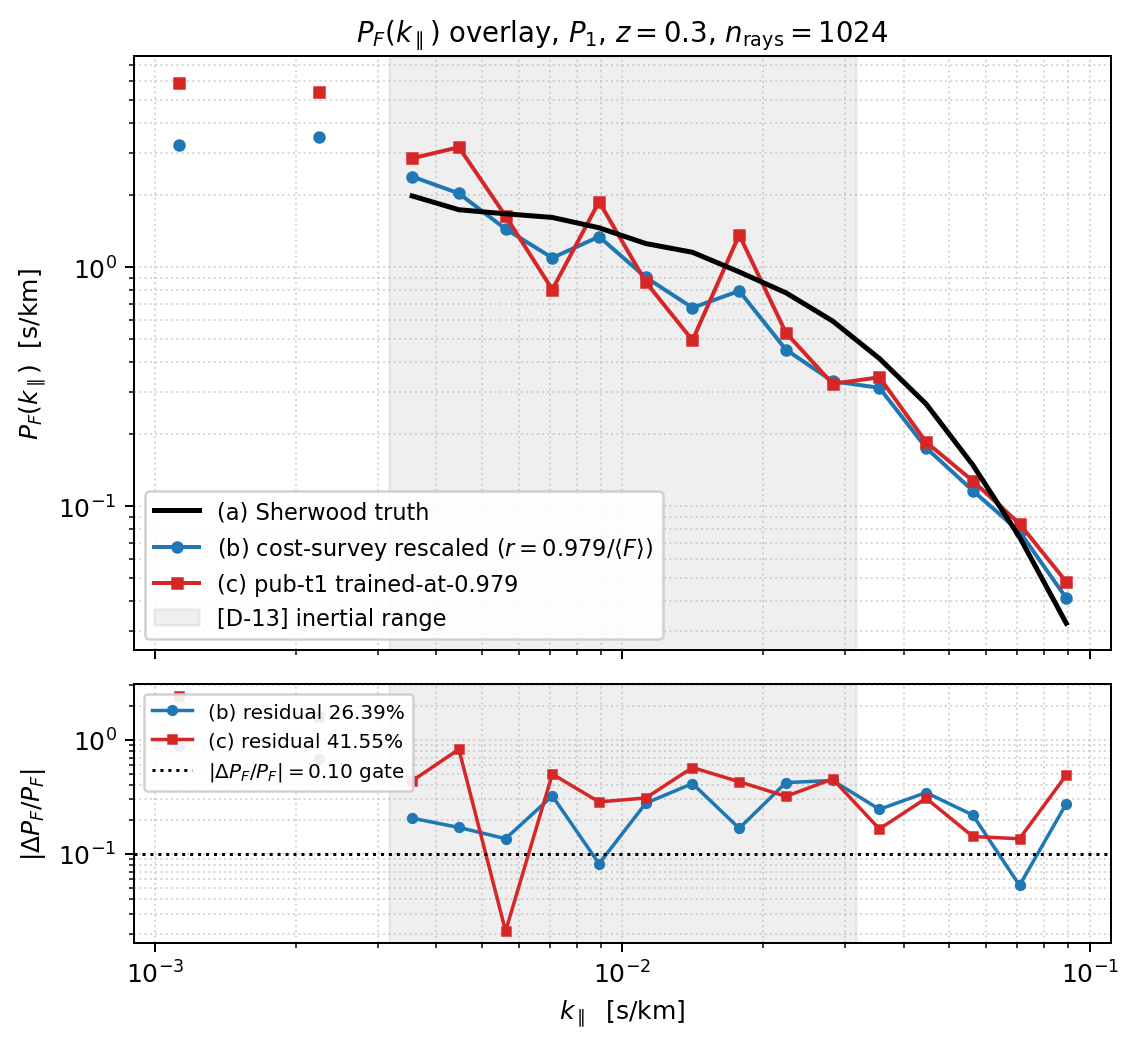
\includegraphics[width=\columnwidth]{figures/pf_overlay_falsification.png}
    \caption{$P_F(k_\parallel)$ overlay at $P_1$, $z{=}0.3$, $n_\mathrm{rays}{=}1024$, eval seed $=42$. Curves: (a) Sherwood ground truth, (b) cost-survey checkpoint after uniform rescale to $\langle F\rangle{=}0.979$ ($|\Delta P_F/P_F|=26.39\%$ under the current normalized-$\delta_F$ pipeline), (c) \texttt{pub-t1} corrected-anchor full-schedule reconstruction ($|\Delta P_F/P_F|=41.55\%$). Shaded band: [D-13] inertial range $k_\parallel \in [10^{-2.5}, 10^{-1.5}]$ s/km; dotted line: $|\Delta P_F/P_F|{=}0.10$ gate. $4\times$ more training and the corrected anchor increased the $P_F$ residual by $\Delta=+15.16$ pp; the shape-vs-scale rescale framework is falsified.}
    \label{fig:pf-overlay-falsification}
\end{figure}

\textbf{Note on the cost-survey checkpoint figure.} Fig.~\ref{fig:p-flux-fiducial}, Fig.~\ref{fig:flux-pdf-fiducial}, and Fig.~\ref{fig:proxy-xi-1d-sample} were generated against the cost-survey T3 checkpoint, on which the rescale-preview framework was originally read. They are retained as the schedule-A reference for the falsification: the rescaled-preview $P_F$ residual at $P_1$ is $26.39\%$ under the current pipeline (Fig.~\ref{fig:p-flux-fiducial}, $31.0\%$ pre-rescale); the trained-at-target $\texttt{pub-t1}$ $P_F$ residual at the same fiducial cell is $41.55\%$ (Tab.~\ref{tab:pub-t1-gates}). All $P_F$ residuals quoted in this paper use the post-fix normalized $\delta_F = F/\langle F\rangle - 1$ convention from \texttt{src/analysis/p\_flux.py}; the [D-35] historical-record value $28.25\%$ for the same statistic is preserved in the LEDGER as the pre-fix-convention reading.

\begin{figure}[t]
    \centering
    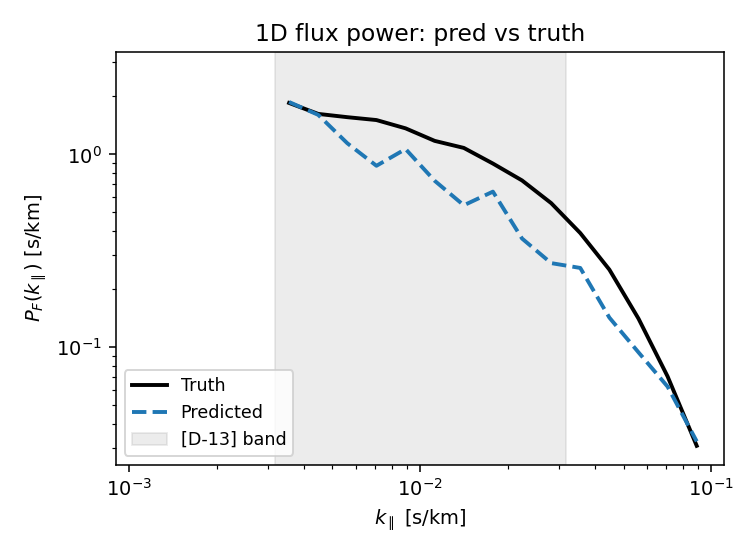
\includegraphics[width=\columnwidth]{figures/d13_pf_fiducial.png}
    \caption{$P_F(k_\parallel)$ reconstruction vs.\ truth at the fiducial point ($P_1$, $z=0.3$, $n_{\text{rays}}=1024$), Tier-3 cost-survey checkpoint (step $10{,}000$). Shaded band marks the [D-13] inertial range $k_\parallel \in [10^{-2.5}, 10^{-1.5}]$ s/km. Mean fractional residual in the inertial range: $\mathbf{31.0\%}$ (gate $<\!10\%$, broken-anchor checkpoint; $26.39\%$ under the [D-35] uniform rescale to the corrected anchor $0.979$ as re-rendered by the current pipeline, retracted as preview by [D-39]). The corrected-anchor full-schedule \texttt{pub-t1} measurement at the same fiducial cell gives $|\Delta P_F/P_F|=41.55\%$ (Tab.~\ref{tab:pub-t1-gates}): $4\times$ more training did not reduce the residual.}
    \label{fig:p-flux-fiducial}
\end{figure}

\begin{figure}[t]
    \centering
    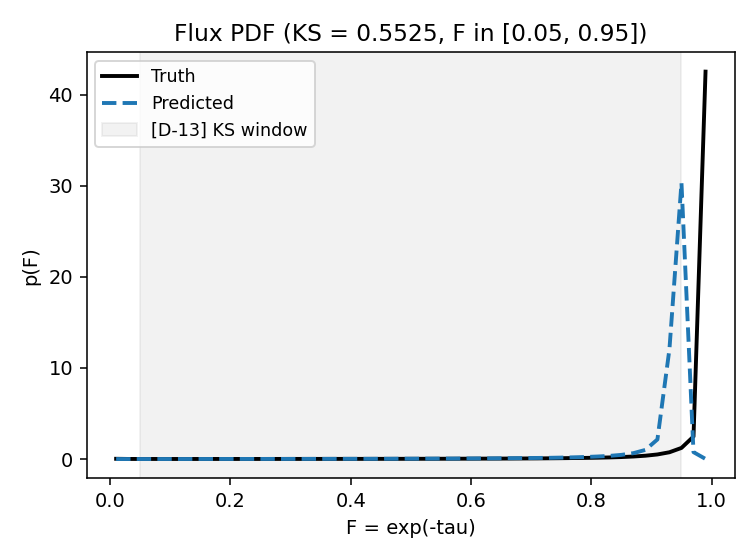
\includegraphics[width=\columnwidth]{figures/d13_flux_pdf_fiducial.png}
    \caption{Flux PDF predicted vs.\ ground-truth, fiducial point, Tier-3 cost-survey. KS distance (cuts $F\in[0.05, 0.95]$): $\mathbf{0.553}$ on the broken-anchor checkpoint, $0.039$ after the [D-35] rescale to the corrected anchor (gate $<\!0.05$, PASS post-rescale; the rescale-as-preview reading is retracted by [D-39]). The corrected-anchor full-schedule \texttt{pub-t1} bundle measures KS$=0.0325$ at $P_1$ and PASSes the gate in $3/4$ cells (Tab.~\ref{tab:pub-t1-gates}); the flux PDF closes while $P_F$ does not.}
    \label{fig:flux-pdf-fiducial}
\end{figure}

\begin{figure}[t]
    \centering
    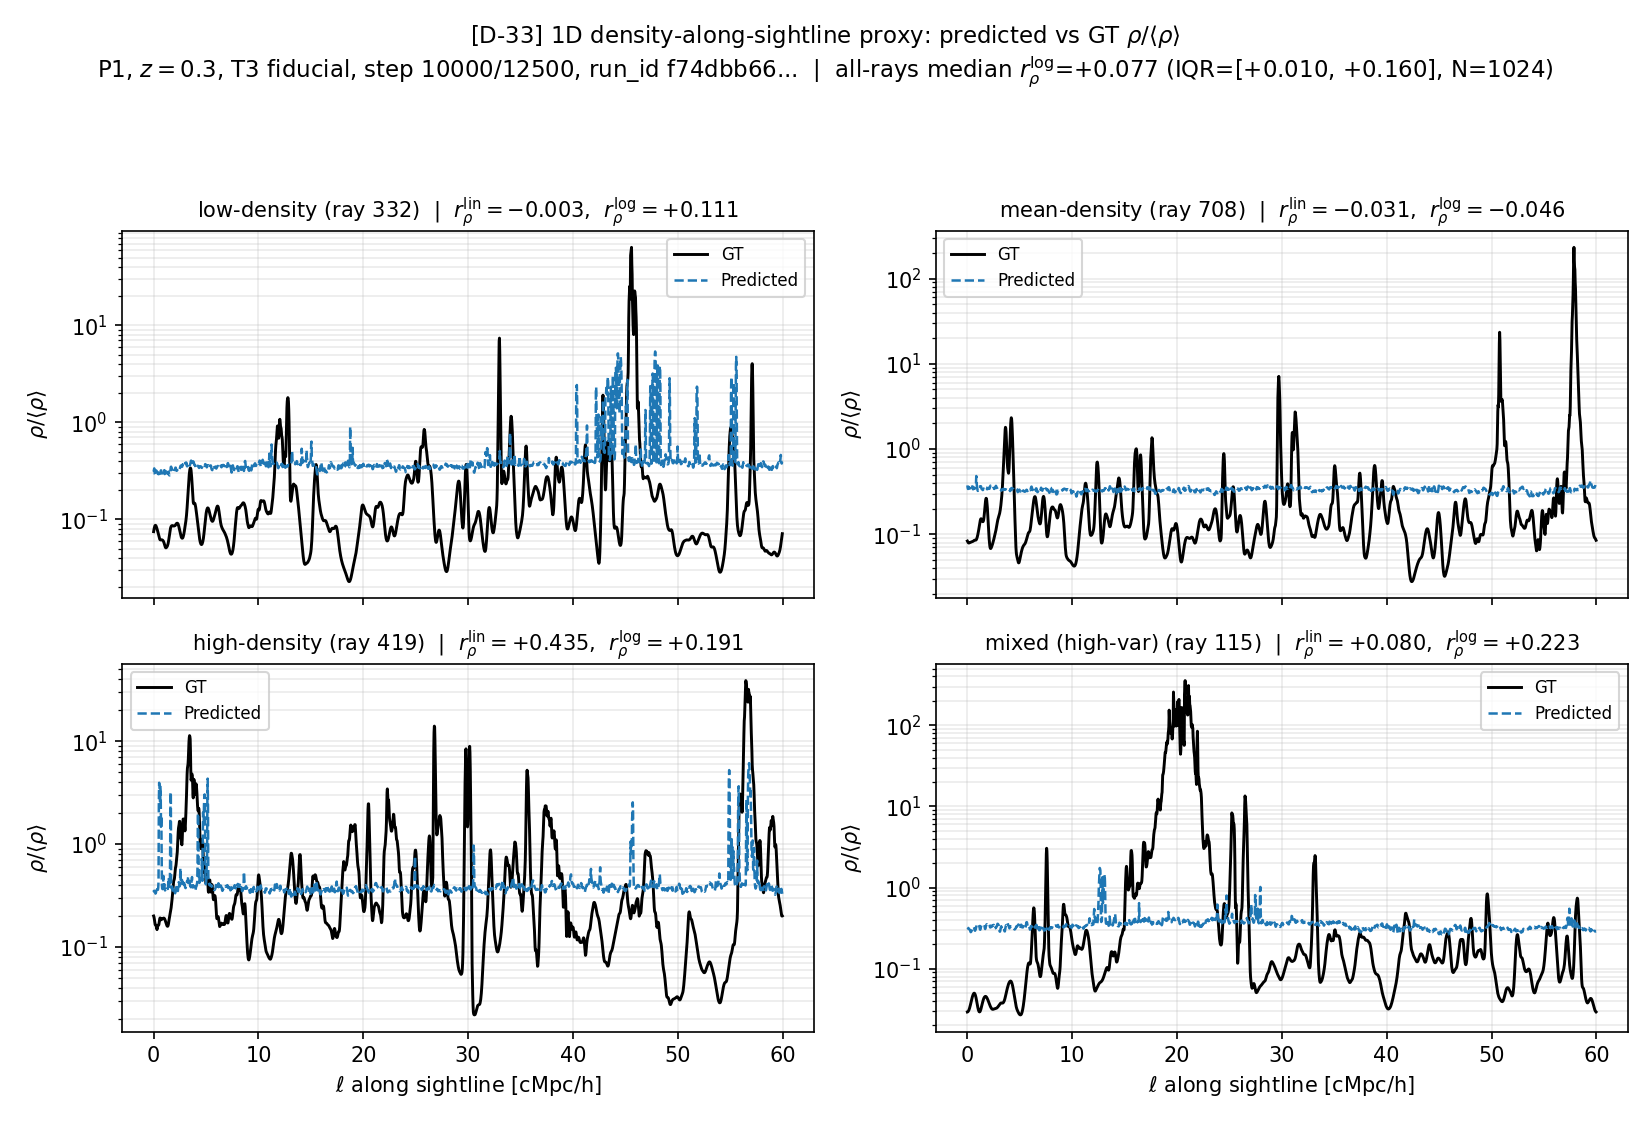
\includegraphics[width=\columnwidth]{figures/proxy_xi_1d_sample.png}
    \caption{\textbf{[D-33] 1D density-along-sightline proxy at T3-$P_1$ fiducial, step $10{,}000/12{,}500$.} Predicted (dashed blue) vs.\ ground-truth (solid black) $\rho/\langle\rho\rangle$ along four representative validation sightlines (low / mean / high density and high-variance), sampled at integrator quadrature points (run\_id \texttt{f74dbb669c\dots}, $P_1$, $z=0.3$, $N=1024$ sightlines). Median per-sightline Pearson correlation on $\log_{10}\rho/\langle\rho\rangle$ is $\mathbf{+0.077}$ (IQR $[+0.010, +0.160]$; 16/84 quantiles $[-0.017, +0.193]$), with $16\%$ of sightlines showing negative correlation --- far below the $\sim 0.6$ CLAMATO-style reconstruction bar~\cite{lee2015}. The proxy is necessary but not sufficient for the deferred 3D $\xi_{\hat\rho,\rho}$ gate; failing it at this schedule is a strong negative signal under the [D-23] cost-survey framing.}
    \label{fig:proxy-xi-1d-sample}
\end{figure}

\begin{table}[t]
    \centering
    \renewcommand{\arraystretch}{1.15}
    \setlength{\tabcolsep}{3pt}
    \footnotesize
    \begin{tabular}{l|c|c|c|c}
    Gate & Pass cond. & Cost-survey (T3, 10k) & Cost-survey rescaled ($r=0.979/\langle\hat F\rangle$) & \texttt{pub-t1} measured ($P_1$, 50k) \\
    \hline
    $|\Delta P_F/P_F|$ (inertial range) & $< 10\%$ & $31.03\%$ (FAIL $3.1\times$) & $26.39\%$ (FAIL $2.6\times$) & $\mathbf{41.55\%}$ (\textbf{FAIL} $\mathbf{4.2\times}$) \\
    KS distance, $F$-PDF & $< 0.05$ & $0.553$ (FAIL $11\times$) & $\mathbf{0.039}$ (PASS) & $\mathbf{0.0325}$ (\textbf{PASS}) \\
    $r_\rho^{\log}$ (1D-proxy [D-33])$^\dagger$ & $> 0.6$ & $+0.077$ (FAIL $\sim 8\times$) & $+0.077$ (anchor-invariant) & (owed: \S\ref{sec:experiments:open-axes}) \\
    \end{tabular}
    \caption{\textbf{[D-13] structure-gate evaluation at the $P_1$ fiducial point, three checkpoints.} \emph{Superseded by [D-39]; rescaled column retained as upper-bound optimism that the trained \texttt{pub-t1} result falsifies.} Cost-survey column: T3 step $10{,}000/12{,}500$ from run \texttt{f74dbb669c\dots} trained against broken anchor $0.877$. Rescaled column: uniform $\hat{F} \to (0.979/\langle\hat{F}\rangle)\cdot\hat{F}$ applied post-hoc, read by [D-35] as a partial preview of the corrected-anchor publication run; [D-35]-era historical cross-physics range (P1/P2/P4) under this rescale, under the pre-fix mean-subtracted $\delta_F$ convention, was KS $\in\{0.039, 0.069, 0.022\}$ (2/3 PASS) and $P_F\in\{28.25\%, 26.50\%, 43.07\%\}$ (0/3 PASS); the $P_1$ entry re-renders to $26.39\%$ under the current normalized-$\delta_F$ pipeline (see footnote in \S\ref{sec:experiments:cosmological-eval} and Fig.~\ref{fig:pf-overlay-falsification}). \texttt{pub-t1} measured column: $P_1$ at the corrected-anchor full-schedule run (step $50{,}000$, run \texttt{31acdf9d\dots}; full four-physics table in Tab.~\ref{tab:pub-t1-gates}). \textbf{Verdict ([D-39]): the rescaled-preview interpretation is falsified.} $4\times$ more training and the corrected anchor increased the $P_F$ residual at $P_1$ from $26.39\%$ to $41.55\%$; the shape-vs-scale hypothesis the rescale framework implied is contradicted by direct measurement. $P_F$ is the binding gate of any successor run. \emph{Implementation note:} $\delta_F$ in \texttt{src/analysis/p\_flux.py} prior to [D-35] used mean-subtraction $F-\langle F\rangle$, which makes $P_F$ scale by $r^2$ under uniform $F\to rF$ (and is therefore not anchor-invariant); the rescaled and \texttt{pub-t1} columns reported here use the post-fix normalized convention $\delta_F = F/\langle F\rangle - 1$, under which $P_F$ is anchor-invariant. $^\dagger$1D-along-ray proxy: per-sightline Pearson $r$ on $\log_{10}\rho/\langle\rho\rangle$ at integrator quadrature points; \emph{necessary but not sufficient} for the deferred 3D $\xi_{\hat\rho,\rho}(r)$ (which requires \texttt{SherwoodIGM\_gal} extracted, $\sim 40$ GB to Juno; deferred per [D-23]). The $> 0.6$ bar is the CLAMATO-style Wiener-filter reconstruction threshold~\cite{lee2015}.}
    \label{tab:d13-gates}
\end{table}

\begin{table}[t]
    \centering
    \renewcommand{\arraystretch}{1.15}
    \setlength{\tabcolsep}{3pt}
    \footnotesize
    \begin{tabular}{l|cccccc}
    Cell & $\langle F_{\text{pred}}\rangle$ & KS ($<\!0.05$) & $|\Delta P_F/P_F|$ ($<\!0.10$) & [D-19] & $\mathcal{L}_{\text{data}}$ (final) & verdict \\
    \hline
    $P_1$ (no fdbk)    & $0.97895$ & $0.0325$ (PASS) & $\mathbf{0.4155}$ (FAIL $\mathbf{4.2\times}$) & PASS & $1.27\!\times\!10^{-7}$ & FAIL on $P_F$ \\
    $P_2$ (wind)       & $0.97536$ & $\mathbf{0.0742}$ (FAIL $1.5\times$) & $\mathbf{0.3757}$ (FAIL $\mathbf{3.8\times}$) & PASS & $1.84\!\times\!10^{-4}$ & FAIL on $P_F$, KS \\
    $P_3$ (wind+AGN)   & $0.97819$ & $0.0408$ (PASS) & $\mathbf{0.3591}$ (FAIL $\mathbf{3.6\times}$) & PASS & $4.14\!\times\!10^{-6}$ & FAIL on $P_F$ \\
    $P_4$ (strong AGN) & $0.98154$ & $0.0389$ (PASS) & $\mathbf{0.3613}$ (FAIL $\mathbf{3.6\times}$) & PASS & $1.28\!\times\!10^{-5}$ & FAIL on $P_F$ \\
    \end{tabular}
    \caption{\textbf{[D-13] structure gates at the corrected-anchor full publication schedule, four feedback variants ([D-39]).} Configuration: \texttt{pub-t1}, $n_{\text{rays}}=64$, \texttt{max\_steps}$=50{,}000$, \texttt{microbatch}$=1024$, \texttt{accum\_steps}$=1$, seed $=0$, $\langle F\rangle_{\text{obs}}=0.979$ (Kirkman+~\cite{kirkman2007}, [D-34] anchor). MLflow run IDs: \texttt{31acdf9d\dots} ($P_1$), \texttt{f7fafa23\dots} ($P_2$), \texttt{62aeb93a\dots} ($P_3$), \texttt{fc3817b3\dots} ($P_4$); tag \texttt{juno\_batch=pub-t1} on Juno a30, ExitCode 0:0 in all four. \textbf{Mean-flux: PASS $4/4$, cross-physics spread $0.63\%$ ($<\!1\%$ bar). KS: PASS $3/4$. $P_F$: PASS $0/4$, uniformly $3.6\times$--$4.2\times$ over the $0.10$ gate.} The $P_F$ residual is the binding gate at the corrected anchor, the full schedule, and four independent feedback variants; the failure is structural and not calibration-bound (mean-flux closes), not seed-collapse (three non-collapsed cells fail $P_F$ at $3.6\times$--$3.8\times$), and not data-MSE-bound ($\mathcal{L}_{\text{data}}$ spans four orders of magnitude across cells without correspondingly resolving $P_F$). \texttt{peak\_vram}$=2.84$ GB in all four; \texttt{tau\_amp} $\in[1.045, 1.117]$; no NaN. Falsifies the [D-35] rescale-as-preview interpretation: \texttt{pub-t1} $P_1$ $P_F=0.4155$ is $\sim\!57\%$ \emph{larger} than the rescaled-preview estimate $0.2639$ at the same anchor (Tab.~\ref{tab:d13-gates}; [D-35]-era historical value $0.2825$).}
    \label{tab:pub-t1-gates}
\end{table}

\begin{table}[t]
    \centering
    \renewcommand{\arraystretch}{1.15}
    \setlength{\tabcolsep}{4pt}
    \begin{tabular}{l|cccc}
    Physics & T1 ($n_{\text{rays}}=64$) & T2 ($256$) & T3 ($1024$) & T4 ($16{,}384$) \\
    \hline
    P1 (no fdbk)       & 0.9282 / 1.224 & 0.9282 / 1.0077 & 0.9283 / 0.9947 & --- \\
    P2 (wind)          & 0.9247 / 2.315 & 0.9266 / 1.0296 & 0.9269 / 1.0215 & --- \\
    P3 (wind+AGN)      & 0.9275 / 2.038 & 0.9272 / 1.0204 & 0.9271 / 1.0255 & --- \\
    P4 (strong AGN)    & 0.9308 / 1.955 & 0.9302 / 1.0288 & 0.9307 / 1.0217 & --- \\
    \end{tabular}
    \caption{Sightline-density $\times$ physics-feedback degradation matrix. Each cell reports \texttt{mean\_flux\_pred} / \texttt{tau\_amp} at the production schedule (50{,}000 steps for T1; 25{,}000 steps for T2; 12{,}500 steps for T3 per [D-23]); all twelve cells PASS the [D-19] safety rails. Source: LEDGER \S6 cost-survey tables under the [D-24] log1p+cap+mask loss. Cross-physics inter-cell mean-flux spreads tighten with rising sightline density: $0.66\%$ (T1) $\to$ $0.39\%$ (T2) $\to$ $0.41\%$ (T3). Tier 4 is currently blocked on the Wrinkle-1 diagnostic ([D-39]; Sec.~\ref{sec:experiments:compute}, Sec.~\ref{sec:nextsteps:tier4}). The three [D-13] gates that consume these checkpoints --- $P_F(k_\parallel)$, $\xi_{\hat\rho,\rho}$, KS-distance --- are reported in Sec.~\ref{sec:experiments:cosmological-eval} against the corrected-anchor \texttt{pub-t1} bundle (Tab.~\ref{tab:pub-t1-gates}); these cost-survey cells are calibration evidence for the per-tier training schedule, not the science gates. \emph{Note:} training used $\langle F\rangle_{\text{obs}}=0.877$ at $z=0.3$, retracted in [D-34] (verified value $0.979\pm 0.005$, \cite{kirkman2007}). \texttt{mean\_flux\_pred} and $\tau_{\text{amp}}$ absolute values are accordingly uninterpretable; inter-cell consistency and the [D-13] structure gates are anchor-invariant per the [D-11] sub-clause and survive unchanged.}
    \label{tab:ablation-matrix}
\end{table}

\subsection{$\tau$-binned residual decomposition: saturation-regime under-fitting, positively identified cross-physics}
\label{sec:experiments:tau-binned}
The structural-$P_F$ verdict of Sec.~\ref{sec:experiments:cosmological-eval} states \emph{that} the gap is in second-order spectroscopic statistics and \emph{not} in calibration; the diagnostic question is \emph{where on the $F$ axis} the gap lives. We answer this with a $\tau$-binned residual decomposition (\texttt{scripts/tau\_binned\_residual.py --cell all}) over the four \texttt{pub-t1} corrected-anchor checkpoints at step $50{,}000$, seed $=42$, $1024$ rays. The diagnostic partitions the rendered $F$ axis into seven bins matching the [D-24] saturated-absorber definition --- linear regime $F > 0.9$ (bins 1--4, $\sim\!99.6\%$ of pixels), transition band, and saturation band $F \in [0.05, 0.30]$ (bin 7) --- and reports the per-bin residual mass $\sum |\Delta F|$ alongside the pixel share, from which the concentration ratio $R = (\text{residual-mass share}) / (\text{pixel-mass share})$ measures how much of the per-sightline error budget the saturation band absorbs relative to its size.

\textbf{Headline.} The saturation-band $R$ is $\{18.87, 19.10, 20.47, 23.75\}$ across $P_1$/$P_2$/$P_3$/$P_4$ (Tab.~\ref{tab:tau-binned-R}, Fig.~\ref{fig:all-residual}). All four cells exceed the positive-ID floor $R \geq 1.5$ by $> \!12\times$, the cross-physics spread is $\sim\!25\%$ relative, and $P_4$ (strongest-feedback variant, where cool dense structure is most prevalent) has the largest $R$. The linear regime contributes $|\langle \Delta F\rangle| \leq 0.03$ across all four cells, so the cross-physics flux residual budget is dominated by the saturation band rather than spread across the $F$ axis. Within the saturation band, the per-bin Pearson $r$ on $\tau$ between predicted and ground-truth values is $r_{\text{pearson}}(\tau) = -0.016$ at $P_1$: the $\tau$-rank order collapses where it matters most for $P_F$, ruling out a global $\tau$ rescaling (uniform $\tau \to s \cdot \tau$ preserves rank order in-band) as a sufficient fix.

\textbf{Interpretation under [D-37].} The decomposition positively identifies the saturation regime as the residually-supported mechanism cross-physics. We do not claim closure of the inferential gap: the strict ``saturation under-fitting \emph{is the cause} of the $P_F$ gap'' claim is reserved for the successor counterfactual run --- a model trained with a saturation-aware loss whose post-hoc $P_F$ residual we can compare directly to the current bundle (Sec.~\ref{sec:nextsteps:pf}). The current claim ceiling is therefore \emph{positively identified as the residually-supported mechanism cross-physics; counterfactual closure (saturation-aware loss) deferred to successor work}.

\textbf{Complementarity to the $P_F$ overlay.} The $P_F$-domain overlay (Fig.~\ref{fig:pf-overlay-falsification}, cost-survey rescaled-preview vs.\ \texttt{pub-t1} measured at fiducial $P_1$) shows the calibration-vs-structure falsification in the spectral domain; the $\tau$-binned figure here shows where on the $F$ axis the unmodeled mass concentrates. The two views are complementary: the $P_F$ overlay diagnoses \emph{that} the failure is structural; the $\tau$-binned decomposition diagnoses \emph{where} it lives.

\begin{figure*}[t]
    \centering
    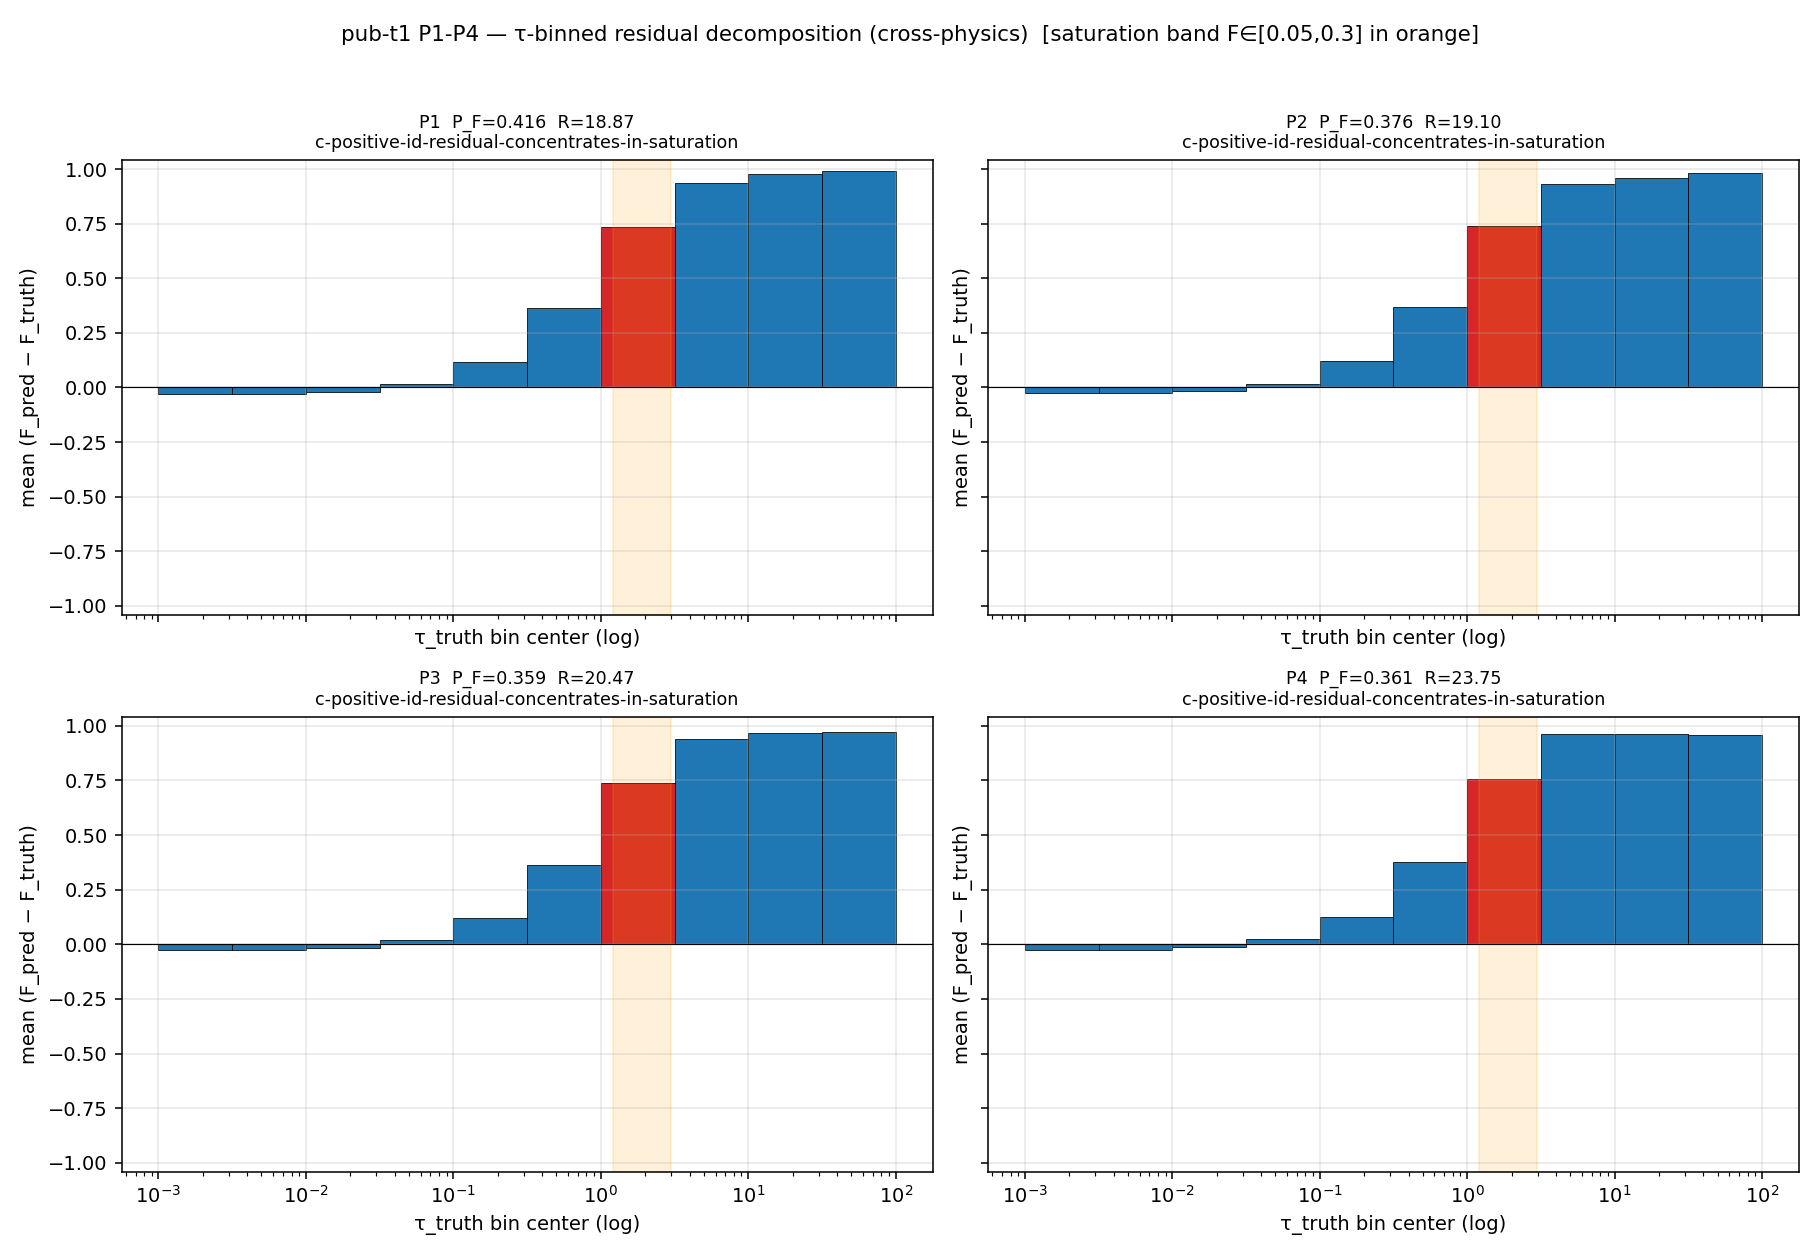
\includegraphics[width=\textwidth]{figures/tau_binned_all_residual.png}
    \caption{\textbf{$\tau$-binned residual decomposition across all four Sherwood feedback variants, positively identifies saturation-regime under-fitting cross-physics.} Configuration: \texttt{pub-t1} corrected-anchor full-schedule checkpoints at step $50{,}000$, seed $=42$, $n_{\text{rays}}=1024$, $\langle F\rangle_{\text{obs}}=0.979$~\cite{kirkman2007}. Each panel: per-bin residual mass $\sum|\Delta F|$ (bars) vs.\ pixel-mass share (dashed) across the seven $F$-bins of the [D-24] saturated-absorber partition; shaded region marks the saturation band $F \in [0.05, 0.30]$. Saturation-band concentration ratios are $R = 18.87$ ($P_1$), $19.10$ ($P_2$), $20.47$ ($P_3$), $23.75$ ($P_4$); positive-ID floor is $R \geq 1.5$; observed range is $\mathbf{18.87}$--$\mathbf{23.75}$ (cross-physics spread $\sim\!25\%$ relative), \textbf{PASS in 4/4 cells} by $>\!12\times$ the floor. Linear regime $F > 0.9$ (bins 1--4, $\sim\!99.6\%$ of pixels) contributes $|\langle \Delta F\rangle| \leq 0.03$ per cell. Within the saturation band, Pearson $r_{\text{pearson}}(\tau) = -0.016$ at $P_1$ --- $\tau$-rank order collapses where it matters most for $P_F$, ruling out a uniform $\tau$ rescaling as a sufficient fix. Verdict: the saturation regime is \emph{positively identified as the residually-supported mechanism cross-physics}; counterfactual closure via a saturation-aware loss term (Sec.~\ref{sec:nextsteps:pf}) is deferred to successor work. Strongest-feedback $P_4$ shows the largest $R$, consistent with the saturation deficit intensifying where cool dense structure is most prevalent. Source: \texttt{experiments/nerf/artifacts/eval/tau\_binned/all\_residual.png}, driver \texttt{scripts/tau\_binned\_residual.py --cell all}.}
    \label{fig:all-residual}
\end{figure*}

\begin{table}[t]
    \centering
    \renewcommand{\arraystretch}{1.15}
    \setlength{\tabcolsep}{6pt}
    \begin{tabular}{l|cc|c}
    Cell & $|\Delta P_F/P_F|$ & $R$ (sat band) & call \\
    \hline
    $P_1$ (no fdbk)     & 0.4155 & 18.87 & PASS positive-ID \\
    $P_2$ (wind)        & 0.3757 & 19.10 & PASS positive-ID \\
    $P_3$ (wind+AGN)    & 0.3591 & 20.47 & PASS positive-ID \\
    $P_4$ (strong AGN)  & 0.3613 & 23.75 & PASS positive-ID \\
    \end{tabular}
    \caption{\textbf{Saturation-band concentration ratio $R$ over the four \texttt{pub-t1} cells.} $R = (\text{residual-mass share})/(\text{pixel-mass share})$ in the saturation band $F \in [0.05, 0.30]$ (bin 7 of the [D-24] partition). Positive-ID floor: $R \geq 1.5$. Verdict: \textbf{PASS in 4/4 cells} by $>\!12\times$; cross-physics range $18.87$--$23.75$ ($\sim\!25\%$ relative spread); $P_4$ (strongest feedback) shows the largest $R$. Configuration: corrected-anchor full schedule (step $50{,}000$, seed $=42$, $n_{\text{rays}}=1024$, $\langle F\rangle_{\text{obs}}=0.979$). The cross-physics $R$-uniformity grounds a single physics-invariant re-weighting scheme in $F \in [0.05, 0.30]$ as the priority successor counterfactual (Sec.~\ref{sec:nextsteps:pf}). The strict ``saturation under-fitting causes the $P_F$ gap'' claim is not made on this evidence: this is the residually-supported mechanism, not closed-loop cause.}
    \label{tab:tau-binned-R}
\end{table}

\textbf{Supplementary view at fiducial $P_1$.} The $P_1$-only single-panel decomposition (\texttt{p1\_residual.png}) is retained as the higher-resolution companion to Fig.~\ref{fig:all-residual} (see supplementary). The single-cell view exposes per-bin $\langle \Delta \tau\rangle$ and $r_{\text{pearson}}(\tau)$ numerics that the four-panel composite compresses for shared-axis comparability; both figures share the same artifact pipeline and pass the same $R \geq 1.5$ gate at $P_1$ ($R = 18.87$). Track-wide $R$-uniformity is the headline; the $P_1$ companion is detail.

\subsection{Open evaluation axes}
\label{sec:experiments:open-axes}
Two evaluation axes remain open against the \texttt{pub-t1} checkpoints and are explicitly not claimed in the structural-$P_F$ verdict of Sec.~\ref{sec:experiments:cosmological-eval}. (a) The [D-33] 1D-along-ray density correlation $r_\rho^{\log}$ has not been re-evaluated on the corrected-anchor checkpoints; the cost-survey value $r_\rho^{\log}=+0.077$ at $P_1$ is anchor-invariant by construction (Tab.~\ref{tab:d13-gates}), but the \texttt{pub-t1} cell is owed for the cross-physics row and is sequenced behind the Wrinkle-1 diagnostic of Sec.~\ref{sec:nextsteps} (shared eval surface; the seed convention may change). (b) The full 3D cross-correlation $\xi_{\hat\rho,\rho}(r=2\,h^{-1}\,\text{Mpc}) > 0.6$ requires the \texttt{SherwoodIGM\_gal} HDF5 particle snapshots ($\sim 40$ GB) for chunked CIC ground-truth reconstruction; the dataset has landed on the Juno scratch tier (LEDGER \S6) and the evaluator is ready, but the gate is gated on a Tier-4 checkpoint that is not in hand.

\subsection{Compute footprint and Tier-4 status}
\label{sec:experiments:compute}
Validation, Tier-1, Tier-2, and Tier-3 production (across four feedback variants on single-GPU NVIDIA Ampere-class hardware, $\geq 12$ GB VRAM) and the four-cell \texttt{pub-t1} corrected-anchor full-schedule bundle have together consumed approximately 62 GPU-hours. The remaining four cells of the production matrix (Tier 4 across the four feedback variants) require an estimated $\sim 792$ GPU-hours, dominated by the $n_{\text{rays}} = 16{,}384$ dense-sightline corner. The implementation is single-GPU-per-job and embarrassingly parallel. Tier 4 is currently \emph{blocked} ([D-39]): dispatching the $\sim 792$-GPU-hr budget is conditional on disambiguating the Wrinkle-1 rescale-vs-trained divergence (Sec.~\ref{sec:nextsteps}), which determines whether sightline density is even the right axis to scale next. The current evidence does not support a hypothesis that sightline density alone closes a $3.6\times$--$4.2\times$ $P_F$ residual. Per-cell GPU-hour breakdown is given in the reproducibility appendix.
